\documentclass[a4paper,11pt,oneside]{book}
\synctex=1

\usepackage{packages}
\usepackage{frontespizio}
%\makeindex                                          %CREA INDICE ANALITICO

%Document begin
\begin{document}
	%\pagenumbering{roman} %IMPOSTA NUMERAZIONE ROMANA FINO ALL'INTRODUZIONE
	%\afterpage{\cfoot{\thepage}} %METTE I NUMERI DI PAGINA IN FONDO AL FOOTER. NECESSARIO SE SI USA FANCYHDR
	\frontespizio
	%\clearpage{\pagestyle{empty}\cleardoublepage}
	%\setlength{\parskip}{0em}
	\tableofcontents
	%\setlength{\parskip}{1em}
	%\newpage
	%\listoffigures
	\newpage
	%\pagenumbering{arabic} %IMPOSTA NUMERAZIONE TRADIZIONALE A PARTIRE DALL'INTRODUZIONE
	%\pagebreak
	%===========================

	% Numeri vicino alla riga
	% @TODO Rimuovere dopo le correzioni
	\linenumbers

	% \onehalfspacing

	% Introduzione
	% !TEX root=../index.tex

\section{Introduzione}
\label{sec:Introduzione}
    Introduzione di carattere generale: human sensing, visione artificiale, importanza delle soluzioni di rilevamento umano e contesti applicativi.

    Stato dell'arte di ampio spettro: face-detection, pedestrian-detection, ecc

    Obiettivo: riferimenti a \cite{Zhu13}, vantaggi del setup top-down

    \cite{Zhu13}

    Setup: descrizione del setup hardware e software

    Presentazione della tesi: descrizione puntuale dei capitoli successivi


	% !TEX root=../index.tex

\chapter{Panoramica del sistema}
\label{cap:overview}
Riproducendo la configurazione proposta in \cite{Zhu13} al soffitto del laboratorio è stato fissato un dispositivo Kinect V2 rivolto verso il pavimento.
In tale configurazione, all'ingresso di una persona nella visuale del Kinect, ne saranno ben visibili la testa e le spalle.

\section{Il Kinect}
\label{sec:sensor}
Ad onor del vero, ciò che viene comunemente chiamato \emph{sensore di profondità} (o sensore di distanza) del Kinect, è in realtà uno \emph{scanner 3D a luce strutturata}\footnote{Nonostante ciò, lo si continuerà a chiamare \emph{sensore di profondità}, leggermente inesatto, ma decisamente più breve ed intuitivo}.
\begin{wrapfigure}{r}{}
    \begin{center}
        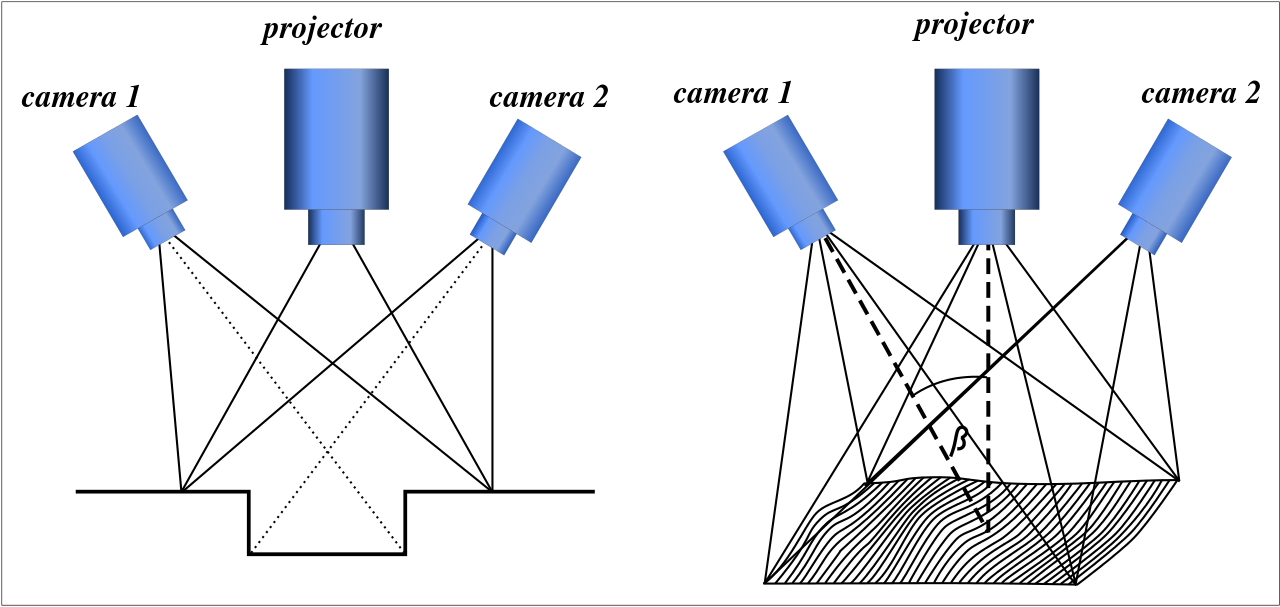
\includegraphics[width=8cm]{img/3d-structured-light-scanner.png}
    \end{center}
    \label{fig:structured_light_scanner}
    \caption{Schematizzazione di uno scanner 3D a luce strutturata.}
\end{wrapfigure}
Un sorgente di raggi infrarossi proietta una serie di pattern codificati. La deformazione indotta dalle superfici degli oggetti interessati viene acquisita da una o più telecamere ed utilizzata per il calcolo delle coordinate tridimensionali.

Il risultato di un sensore di questo tipo è un insieme di triplette $(x,y,z)$, organizzate in una \emph{immagine di profontità}, una struttura dati che è molto simile ad una semplice immagine in scala dei grigi, dove il valore di ogni pixel rappresenta la misura in millimetri della distanza della superficie dal sensore.
La forte somiglianza con le immagini in scala dei grigi è supportata dal fatto che ogni pixel è codificato utilizzando 16bit.

La massima affidabilità del sensore del Kinect si ha per distanza comprese tra $50cm$ e $4,5m$.
Il dispositivo è montato al soffitto a $2,8m$ da terra e ha un campo visivo di $70^{\circ} \times 60^{\circ}$, il quale, all'altezza del pavimento, determina un'area di cattura di circa $4m \times 5m$.

La dimensione di ogni immagine di profondità è di $512 \times 424$ pixel. Nativamente non vengono codificate in alcun modo particolare, sono delle semplici matrici di interi.
Il Kinect V2 è in grado di catturarne fino a 30 al secondo. Utilizzando un apposito software di registrazione è stato possibile mettere insieme dei video di profondità a 30 fps.

\section{Head and Shoulder Profile}
\label{sec:hasp}

\begin{wrapfigure}{l}{}
    \begin{center}
        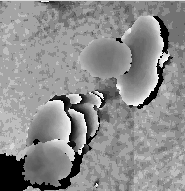
\includegraphics[width=5cm]{img/no_occlusion.png}
    \end{center}
    \caption{Due persone in un ritaglio proveniente da un frame di profondità. Il frame è stato acquisito con il Kinect V1, a differenza di quello in figura \ref{fig:spatial_feature}, acquisito con il Kinect V2.}
    \label{fig:no_occlusion}
\end{wrapfigure}

In condizioni ottimali, la figura umana ripresa dall'alto è composta solamente dalla testa e dalle spalle.
Finchè si trova quasi in corrispondenza del sensore, nella parte centrale dell'immagine di profondità, la restante parte del corpo rimane quasi del tutto nascosta. Sulla posizione delle braccia non si possono fare delle assunzioni precise.

In figura \ref{fig:no_occlusion}, la figura dell'individuo a destra corrisponde a tale descrizione, mentre dell'altro è visibile parte del corpo ed una delle due spalle è nascosta dalla testa.
Nelle zone periferiche di un frame di profondità, l'immagine è soggetta alla \emph{distorsione prospettica} così come lo è quella di qualunque telecamere RGB.

Tale distorsione costituisce un disturbo, dal momento che la figura dello stesso soggetto varia a seconda della relativa posizione nell'area di visualizzazione.
Si vedrà più avanti come affrontare tale situazione, per il momento si considerano solamente le immagini proveniente dalle zone centrali dei frame (come quella in figura \ref{fig:spatial_feature}).

Un grande vantaggio dell'utilizzo del Kinect in questa configurazione è l'\emph{assenza di occlusione}.
Infatti, rispetto ai molteplici sistemi di riconoscimento frontali, i soggetti non possono nascondersi l'uno con l'altro al sensore.

Utilizzare le immagini di profondità significa ragionare con le distanze: piuttosto che cercare di descrivere l'immagine del profilo umano in termini di forma, deve essere descritto in termini di differenze di quota rispetto all'ambiente circostante.
Alla luce di ciò, si possono identificare i seguenti criteri descrittivi:

\begin{enumerate}
    \item L'immagine di una persona è caratterizzata da uno spazio vuoto di fronte ad essa e dietro di essa. Per \emph{spazio vuoto} si intende una regione la cui distanza dal sensore è circa quella del pavimento.
    \item A sinistra della spalla sinistra ed a destra della spalla destra del profilo dall'alto di una persona, sono presenti degli spazi vuoti.
    \item Tra la testa e le spalle vi è una differenza di altezza.

\end{enumerate}

\begin{wrapfigure}{r}{}
    \begin{center}
        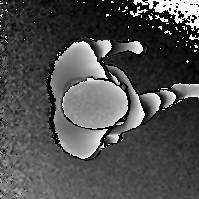
\includegraphics[width=4cm]{img/spatial_features.png}
    \end{center}
    \caption{Una persona mentre cammina}
    \label{fig:spatial_feature}
\end{wrapfigure}

Di qui in avanti, con l'acronimo \emph{HASP} (\emph{Head And Shoulder Profile}), ci si riferirà proprio al profilo della persona ripreso dall'alto che soddisfa i criteri appena elencati.

\section{Un problema di Classificazione} % (fold)
\label{sub:struttura_software}
Il software è diviso in due moduli: il modulo per il riconoscimento e il modulo di allenamento.

Nella prima fase, quella di allenamento, il relativo modulo software, a partire da un insieme di campioni classificati, genererà un insieme di regole per classificare campioni con le medesime caratteristiche. Implementa l'algoritmo Adaboost.

La seconda fase, quella di riconoscimento, lavora su dati reali: ad ogni frame acquisito tramite il sensore di profondità del Kinect si applicano le regole di classificazione generate nella fase precedente, stabilendo se nel frame è stata ripresa una persona e - in caso affermativo - la posizione di quest'ultima.


	% !TEX root=../index.tex

\chapter{Haar-like Features}
\label{cap:haar_features}
\emph{Definizione delle feature.
Derivazione delle feature dalle wavelet di Haar.
Immagini integrali.
Decision Stump.} 


La descrizione di un qualsiasi oggetto avviene attraverso la descrizione dei suoi attributi. La forma geometrica, le dimensioni, il peso, il colore sono solo una manciata dei possibili attributi con i quali descrivere un oggetto.
L'essere umano è dotato di 5 sensi attraverso i quali è in grado di \emph{percepire} la realtà circostante e di un'infinità di modi con cui \emph{descriverla}.

Il riconoscimento di un oggetto avviene solo in un secondo momento, attraverso l'analisi della sua descrizione, valutando gli attributi che, in quel contesto, sono più signicativi.
Nell'ambito della visione artificiale, il riconoscimento degli oggetti segue esattamente lo stesso flusso.
Gli attributi di un oggetto vengono descritti mediante l'utilizzo di \emph{feature}, ovvero dei meccanismi per misurare le varie proprietà dell'oggetto stesso.

Le immagini di profondità sono il frutto della percezione della realtà, le feature di Haar costituiscono gli attributi con i quali è possibile descrivere tali immagini.


\section{Definizione}
\label{sec:haar_def}
Le feature di Haar riescono a misurare la quantità e il verso delle variazioni di intensità tra due regioni adiacenti di una immagine.
La comune rappresentazione grafica di tali feature mette in evidenza le due regioni colorandone una bianco e l'altra di nero.
La somma delle intensità dei pixel della regione bianca a cui viene sottratta la somma delle intensità della regione nera fornisce una misura della variazione media di intensità tra le due regioni (equazione \ref{eq:haar_feature_informal}).

Di feature ne esistono di diverse forme: in figura \ref{fig:features_type} sono presenti quelle utilizzate in questo ambito, ma disponibili molte forme di feature utilizzate da altri sistemi di object detection. Non tutte sono formate solamente da \emph{due regioni adiacenti}, ma l'importante è che tutte abbiano una regione \emph{nera} ed una regione \emph{bianca}.

\begin{wrapfigure}{L}{0cm}
    \centering
    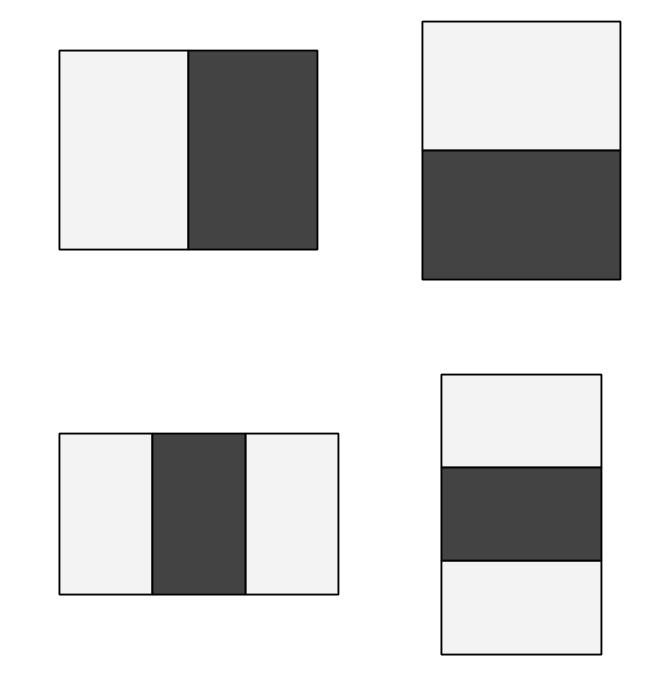
\includegraphics[width=5cm]{img/feature_types.jpg}
    \caption{Tipi di feature di Haar utilizzati in \cite{Zhu13}.}
    \label{fig:features_type}
\end{wrapfigure}

L'equazione \ref{eq:haar_feature_informal} fornisce una descrizione informale del funzionamento delle feature di Haar. Con $E(Area)$ si intende la somma delle intensità di tutti i pixel che appartengono all'area specificata.

\begin{equation}
    f(Img) = E(Area_{white}) - E(Area_{black})
    \label{eq:haar_feature_informal}
\end{equation}

Il segno del valore di una feature identifica il verso della variazione. Se si prende in esame la forma di feature in alto a sinistra della figura \ref{fig:features_type}, un valore positivo denota un'intensità mediamente maggiore nella regione bianca rispetto alla media della regione nera e viceveresa.

Evidenziare le variazioni di intensità delle immagini integrali attraverso l'applicazione delle feature di Haar equivale ad evidenziare le differenze di quota medie delle regioni individuate dalla feature e questo le rende particolarmente adatte a questa applicazione.

In seguito sarà necessario dover calcolare gruppi di feature in diverse scale. Ridimensionare un gruppo di feature è una cosa semplice e verrà trattata in seguito, ma affinchè il valore della feature sia il meno possibile sensibile ai ridimensionamenti è necessario rapportare tale valore all'estensione totale dell'area interessata (equazione \ref{eq:haar_scale_invariant}).

\begin{equation}
    f'(Img) = \frac{E(Area_{white}) - E(Area_{black})}{size(Area_{white}) + size(Area_{black})}
    \label{eq:haar_scale_invariant}
\end{equation}

\section{Dalle Wavelet di Haar alle Feature}
\label{sec:haar_wavelet}
Le feature di Haar derivano dall'estensione bidimensionale delle wavelet di Haar, che sono il primo esempio di wavelet e vennero sviluppate nel 1909 da Alfrèd Haar \cite{Haar10}.
La wavelet madre (equazione \ref{eq:mother_wavelet}) è una funzione oscillante di lunghezza finita, caratteristica comune a tutti i tipi di wavelet.

\begin{equation}
\label{eq:mother_wavelet}
    \psi(x) =
    \begin{cases}
        1 & 0 \leq t < 1/2 \\
        -1 & 1/2 \leq t < 1 \\
        0 & \text{ altrimenti }
    \end{cases}
\end{equation}

Ogni segnale può essere rappresentato per mezzo delle wavelet di Haar. Costituiscono un sistema di rappresentazione duale alla serie di Fourier.

\begin{figure}[!htb]
    \minipage{0.45\textwidth}
    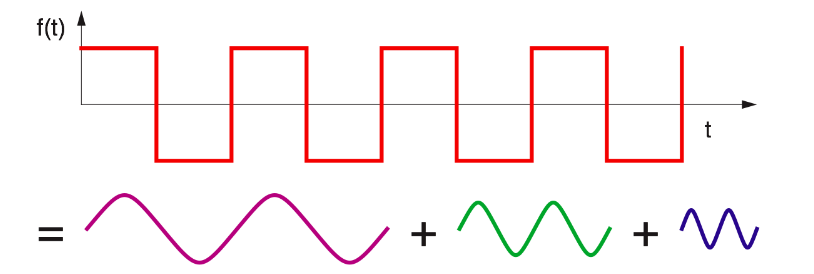
\includegraphics[width=\linewidth]{img/fourier_rapresentation.png}
    \caption{Rappresentazione di un segnale con una serie di funzioni armoniche.}
    \label{fig:awesome_image1}
    \endminipage\hfill
    \minipage{0.45\textwidth}
    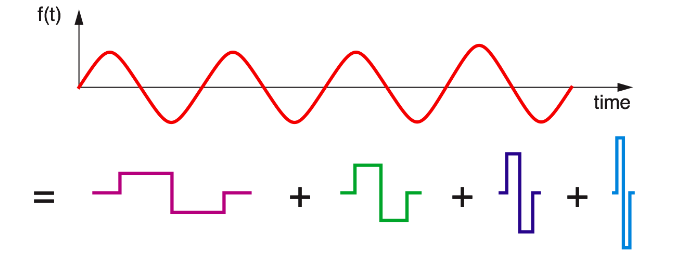
\includegraphics[width=\linewidth]{img/haar_rapresentation.png}
    \caption{Rappresentazione di un segnale con una serie di wavelet di Haar.}
    \label{fig:awesome_image2}
    \endminipage
\end{figure}

Alfrèd Haar propose anche la prima DWT (\emph{Discrete Wavelet Transform}) con la quale, le wavelet che compongono un segnale, vengono campionate discretamente.
Le applicazioni sono notevoli e ad ampio spettro, prime tra tutte quelle nell'ambito della codica dei segnali e nella compressione dei dati. Per fare un esempio, lo standard di compressione JPEG2000 sfrutta la trasformazione DWT \cite{Jpeg2000} per ottenere risultati qualitativamente migliori rispetto allo standard precedente.

Una variante della trasformazione DWT con le wavelet di Haar bidimesionali (figura \ref{sec:haar_wavelet}) è stata utilizzata da \citet{Oren97} in un sistema in grado di riconoscere la presenza di pedoni in delle immagini.

\begin{wrapfigure}{L}{0cm}
    \centering
    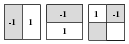
\includegraphics[width=3cm]{img/haar_wavelet.png}
    \caption{Wavelet di Haar bidimensionali utilizzate in \cite{Oren97}.}
    \label{fig:haar_wavelet}
\end{wrapfigure}

Applicando alle immagini la trasformata DWT in diverse scale, si passa da una rappresentazione dell'immagine in scala dei grigi, ad una rappresentazione in termini di coefficienti delle wavelet di Haar.
Tali coefficienti denotano le differenze di intensità tra le aree adiacenti dell'immagine e vengono utilizzati per evidenziare analogie strutturali delle immagini che contengono la figura di un pedone.

\begin{wrapfigure}{R}{0cm}
    \centering
    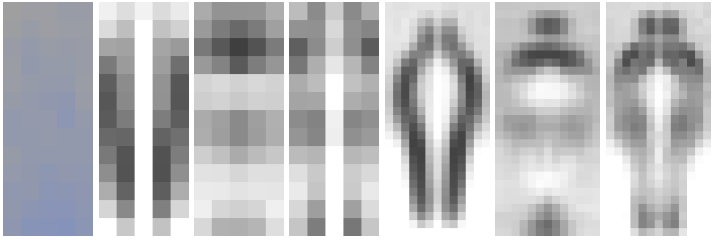
\includegraphics[width=8cm]{img/pedestrian_dwt.png}
    \caption{Coefficienti delle wavelet di trasformate DWT di diverse scale applicate alla stessa immagine. I coefficienti vengono codificati utilizzando la scala dei grigi \cite[Figura 3]{Oren97}.}
    \label{fig:non_standard_dwt}
\end{wrapfigure}

Nella descrizione di un framework generale per l'object detection, \citet{Papageorgiou98} utilizzano la trasformata DWT a wavelet di Haar bidimensionali non per l'estrazione di un template dell'oggetto espresso in variazioni di intensità, bensì per la selezione delle wavelet più significative al fine del riconoscimento dell'oggetto.

Una wavelet di Haar bidimensionale di una data dimensione, utilizzata per campionare un'immagine in una posizione specifica mette in evidenza le differenze di intensità dell'immagine nella regione descritta dall'area della wavelet. Tale differenza di intensità costituisce una proprietà osservabile e misurabile dell'immagine che ritrae l'oggetto. Queste sono le \emph{Haar-like feature} (o semplicemente feature di Haar).

\section{Immagine Integrale}
\label{sec:integral_image}
Le feature di Haar vengono utilizzate anche nel riconoscimento dei volti umani di Viola-Jones.
Sono molto apprezzate, sebbene siano molto primitive rispetto ad altri tipi più evoluti di feature, per la loro efficienza computazionale.

Il calcolo della somma delle intensità dei pixel di un'area è un'operazione il cui costo aumenta linearmente con la quantità di pixel. Introducendo il concetto di \emph{immagine integrale}, ottenuta rielaborando l'immagine di partenza, tale somma viene eseguita una volta per ogni immagine, permettendo in seguito di calcolare il valore di ogni feature in un tempo costante.

\begin{definition}
    Sia $I$ un'immagine larga $w$ pixel ed alta $h$ pixel. Con la scrittura $I(x, y)$ si identifica il pixel dell'immagine $I$ che si trova alla colonna $x$ e alla riga $y$.
    Si definisce \emph{immagine integrale} (altrimenti detta \emph{Summed Area Table}) una seconda immagine $SAT$ delle stesse dimensioni per cui vale $\forall x \in [1,w], y \in [1,h]$:
    \begin{equation}
        SAT(x, y) = \sum_{i = 1}^{x} \sum_{j = 1}^{y} I(i, j)
    \end{equation}
\end{definition}

\begin{wrapfigure}{L}{0cm}
    \centering
    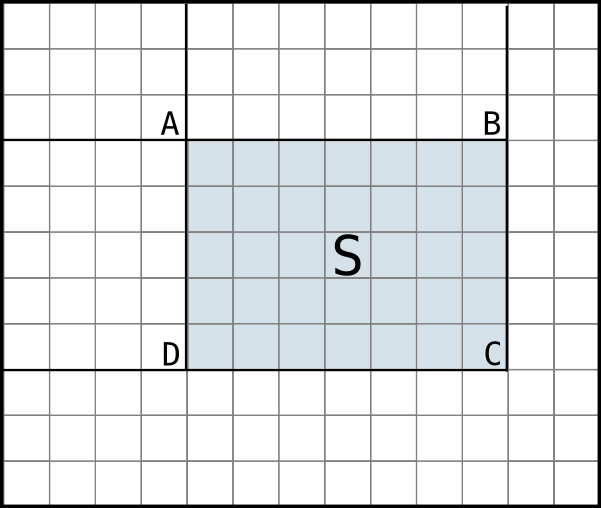
\includegraphics[width=5cm]{img/integral_image_sum.png}
    \caption{}
    \label{fig:integral_image_sum}
\end{wrapfigure}

Calcolare la somma del valore dei pixel contenuti in una regione rettangolare dell'immagine originale, con l'ausilio dell'immagine integrale, è un'operazione velocissima.

Si consideri la figura \ref{fig:integral_image_sum}: si vuole calcolare la somma del valore dei pixel nella regione $S$ evidenziata. I vertici del rettangolo saranno i punti $A:(x_1,y_1)$, $B:(x_2,y_1)$, $C:(x_2,y_2)$, $D:(x_1, y_2)$, notando che $1 \leq x_1 \leq x_2 \leq w$ e che $1 \leq y_1 \leq y2 \leq h$ \footnote{Nelle immagini raster, si iniziano a contare le colonne e le righe dal punto in alto a sinistra.}.
Quindi:

\begin{align*}
    \sum_{i = x_1}^{x_2} \sum_{j = y_1}^{y_2} I(i,j) =
    \sum_{i = 1}^{x_2} \sum_{j = y_1}^{y_2} I(i,j) - \sum_{i = 1}^{x_1} \sum_{j = y_1}^{y_2} I(i,j) = \\
    =
    \left(
    \sum_{i = 1}^{x_2} \sum_{j = 1}^{y_2} I(i,j) -
    \sum_{i = 1}^{x_2} \sum_{j = 1}^{y_1} I(i,j)
    \right)
    -
    \left(
    \sum_{i = 1}^{x_1} \sum_{j = 1}^{y_2} I(i,j) -
    \sum_{i = 1}^{x_1} \sum_{j = 1}^{y_1} I(i,j)
    \right) = \\
    = SAT(C) - SAT(B) - SAT(D) + SAT(A)
\end{align*}

Elaborare l'immagine integrale è un'operazione con complessità computazionale $\Theta(w \cdot h)$, cioè il cui costo varia linearmente con la dimensione dell'immagine. Una volta ottenuta però, permette di calcolare qualsiasi somma di pixel in regioni rettangolari con operazioni di complessità $\Theta(1)$.

Grazie all'immagine integrale è quindi possibile valutare in tempi brevi, gruppi enormi di feature sulla stessa immagine.


\section{Decision Stump}
\label{sec:decision_stump}
\begin{wrapfigure}{R}{0cm}
    \centering
    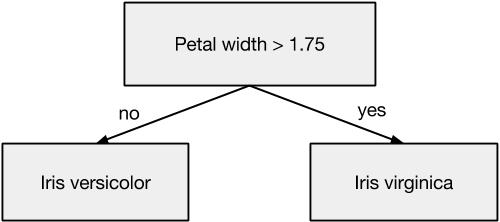
\includegraphics[width=7cm]{img/decision_stump.jpg}
    \caption{Esempio di decision stump usato per dividere gli oggetti in due classi delle tre descritte nel dataset delle caratteristiche dei fiori di Iris \cite{Fisher36}}
    \label{fig:decision_stump}
\end{wrapfigure}
Si tratta di \emph{alberi decisionali} binari di profondità unitaria.
Vi è un unico test alla radice, in base al quale si decide l'appartenenza di un oggetto ad due classi. Combinando tra loro diversi decision stump, è possibile creare alberi decisionali più complessi da poter utilizzare in alberi di classificazione non binari.

I decision stump costituiscono il meccanismo più semplice di classificazione che si può avere a disposizione. Il test da collocare alla radice dell'albero viene eseguito sul valore di una feature di Haar.

\begin{equation}
    test_1(x) =
    \begin{cases}
        true & \text{ se } f_1(x) < \theta_1\\
        false & \text{ altrimenti }
    \end{cases}
    \label{eq:decision_stump_minor}
\end{equation}

\begin{equation}
    test_2(x) =
    \begin{cases}
        true & \text{ se } f_2(x) > \theta_2\\
        false & \text{ altrimenti }
    \end{cases}
    \label{eq:decision_stump_maior}
\end{equation}

Le equazioni \ref{eq:decision_stump_minor} e \ref{eq:decision_stump_maior} descrivono due possibili test decisionali che possono essere collocati alla radice di un decision stump.
Per standardizzare la forma dei test si utilizzerà l'equazione \ref{eq:decision_stump}.

\begin{equation}
    test(x) =
    \begin{cases}
        true & \text{ se } f(x)p > p\theta\\
        false & \text{ altrimenti }
    \end{cases}
    \label{eq:decision_stump}
\end{equation}

In riferimento all'equazione \ref{eq:decision_stump}, $x$ è un'immagine di profondità, $f$ una feature di Haar ed $f(x)$ il valore della feature misurato sull'immagine $x$.
Il parametro $p \in \{ 1, -1 \}$, che assumerà il nome di \emph{polarità}, serve solamente per invertire il segno della disequazione all'occorrenza.
Il parametro $\theta$ è il valore di \emph{soglia} (\emph{threshold}).

Utilizzare i decision stump con le immagini di profondità equavale a verificare la presenza di variazioni di quota tra regioni contigue dell'immagine al di sopra o al di sotto di un certo valore di soglia.
La scelta del valore di soglia non è un problema banale e sarà trattato approfonditamente nel prossimo capitolo.

Il successo o l'insuccesso del test deve essere interpretato correttamente ai fini della classificazione. Di qui in avanti qualsiasi test decisionale applicato ad immagini di profondità che avrà successo, segnalerà la presenza di una persona, mentre, viceversa, quelli che non avranno successo ne segnaleranno l'assenza.


	% !TEX root=../index.tex

\chapter{Adaboost}
\label{cap:adaboost}
\emph{Classificazione nell'ambito degli algoritmi di apprendimento automatico.
Costruzione e preparazione dei dataset di allenamento:
    definizione delle categorie di classificatori da utilizzare;
    operazioni preliminari di preprocessing.
Procedura di estrazione del classificatore forte.
Procedura di estrazione del miglior classificatore debole.}


Adaboost è un algoritmo di apprendimento automatico della famiglia degli \emph{ensamble learner}. Un algoritmo di ensamble learning mira alla costruzione di un classificatore composto da un insieme di


Adaboost è un \emph{meta algoritmo} di \emph{machine learning} che viene utilizzato per aumentare le prestazioni di altri algoritmi di apprendimento. Ciò avviene estraendo un \emph{classificatore forte} a partire da un insieme di \emph{classificatori deboli}, dove per classificatore si intende una funzione $f(x)$ che identifichi la \emph{classe} di appartenenza dell'oggetto $x$ in input.

La realtà d'interesse del problema prevede l'esistenza di due classi di oggetti: \emph{umano} e \emph{non umano}.

I dati in input per la fase di allenamento sono costituiti dal \emph{dataset di allenamento}, ovvero una raccolta di oggetti preclassificati attraverso i quali Adaboost riuscirà a selezionare una combinazione di classificatori deboli che meglio approssimano la classificazione degli elementi del dataset.

\subsection{Il dataset dall'allenamento} % (fold)
\label{sub:il_dataset_dall_allenamento}
La finestra di visualizzazione, come accennato in precedenza è di $512 \times 424$ pixel. In una registrazione che riprende dall'alto una persona che attraversa la stanza camminando, la figura della persona occupa una porzione della finestra di circa $160 \times 100$ pixel.

Un dataset di allenamento non è altro che un insieme di porzioni di frame di una certa dimensione (la stessa per tutti) che vegono classificati manualmente dal creatore\footnote{Il sistema di apprendimento che si sta trattando ricade nella categoria dei sistemi di \emph{apprendimento supervisionato}.} del dataset.

% subsection il_dataset_dall_allenamento (end)

\subsection{Estrazione del classificatore forte} % (fold)
\label{sub:estrazione_del_classificatore_forte}
Sia $D = \{(x_1, y_1), ..., (x_n, y_n)\}$ un insieme di $n$ coppie costituite da un'immagine ($x_i$) e la relativa classificazione ($y_i \in \{ 0, 1 \}$). Se $y_i = 1$, allora $x_i$ appartiene alla classe \emph{umano} (la coppia $(x_i, y_i)$ prende il nome di \emph{esempio positivo}), altrimenti appartiene alla classe \emph{non umano} (la coppia $(x_i, y_i)$ prende il nome di \emph{esempio negativo}).

L'insieme $D$ può essere partizionato come segue:
$$P = \{(x, y) \in D | y = 1\} \text{ e } N = \{(x,y) \in D | y = 0\}$$

Si tenga a mente che, essendo $P$ ed $N$ partizioni di $D$, valgono le seguenti\footnote{La scrittura $\#(D)$ denota il numero di elementi dell'insieme $D$.}:
\begin{equation}
    D = P \cup N
\end{equation}
\begin{equation}
    P \cap N = \emptyset
\end{equation}
\begin{equation}
    \#(D) = \#(P \cup N) = \#(P) + \#(N)
\end{equation}

Si introduce anche il concetto di \emph{classificatore debole}. Si tratta di una funzione che per una data immagine $x$ in ingresso, assume il valore che simboleggia la presunta classe di appartenenza di quest'ultima.
Nel dettaglio:
\begin{equation}
    h(x) = \begin{cases}
    1 & \text{se $pf(x) < p\theta$}\\
    0 & \text{altrimenti}
\end{cases}
\end{equation}
dove $f(x)$ è il valore di una feature di Haar applicata all'immagine $x$, $p \in \{-1,1\}$ è detta \emph{polarità} e $\theta$ è la \emph{soglia} (\emph{threshold}). Tutti i classificatori deboli sono costruiti usando un'unica feature.

L'obbiettivo di Adaboost è quello di formare un \emph{classificatore forte} come combinazione lineare dei migliori classificatori deboli estraibili dal set di allenamento, dove il fattore moltiplicativo di ogni classificatore nella combinazione è inversamente proporzionale agli errori di classificazione compiuti da quest'ultimo in fase di allenamento.

Il seguente algoritmo descrive la procedura di estrazione e combinazone di $T$ classificatori deboli.

\begin{enumerate}
    \item Si associa ad ogni elemento $(x_i, y_i) \in D$ un peso $w_i$ tale che $w_i = \frac{1}{2l}$ se $(x_i, y_i) \in P$ oppure $w_i = \frac{1}{2m}$ se $(x_i, y_i) \in N$, dove $l = \#(P)$ ed $m = \#(N)$ (numero degli esempi positivi e numero degli esempi negativi).

    Sia inoltre $n := \#(D) = \#(P) + \#(N) = l + m$.

    \item \emph{For} $t = [1:T]$
    \begin{enumerate}
        \item Si normalizzano i pesi, in modo che la loro somma sia pari ad 1:
        $$ w_{t,i} \leftarrow \frac{w_{t,i}}{\sum_{j = 1}^{n}w_{t,j}}$$

        \item \label{adaboost_minimum_error}
        Si estrae il miglior classificatore debole. La procedura viene esposta nel dettaglio nella sezione \ref{sub:il_miglior_classificatore_debole}, ma si tenga presente che il miglior classificatore è quello il cui \emph{errore pesato} è minimo per la corrente iterazione.
        $$ \epsilon_t = \min_{f,p,\theta} \{
        \sum_{i = 1}^{n} w_{t,i} \cdot |h(x_i, f, p, \theta) - y_i|
        \} $$
        Siano inoltre $f_t$, $p_t$, $\theta_t$ i parametri del classificatore debole che ne minimizzano l'errore pesato:
        $$ h_t(x) := h(x, f_t, p_t, \theta_t) $$

        \item \label{adaboost_beta} $\beta_t \leftarrow \frac{\epsilon_t}{1 - \epsilon_t}$

        \item \label{adaboost_update_weights} Si aggiornano i pesi
        $$ w_{t+1, i} \leftarrow w_{t,i} \cdot \beta_{t}^{e_i} $$
        dove $e_i = 1$ se $(x_i, h_t(x_i)) \in D$ (ovvero se $x_i$ è classificata correttamente), $e_i = 0$ altrimenti.

        \item $\alpha_t \leftarrow \log(\frac{1}{\beta_t})$
    \end{enumerate}

    \item \label{adaboost_strong_classifier} Il classificatore forte è dato da:
    \begin{equation}
        F(x) = \begin{cases}
        1 & \text{ se } \sum_{t = 1}^{T} \alpha_t h_t(x) > \theta \sum_{t = 1}^{T} \alpha_t \\
        0 & \text{ altrimenti }
    \end{cases}
\end{equation}
dove $\theta \in [0,1]$ è la soglia.
\end{enumerate}

Si noti che, nel'operazione \ref{adaboost_minimum_error}, l'errore pesato non è altro che la somma dei pesi degli esempi non classificati correttamente. Infatti:
$$ h(x_i, f, p, \theta) = y_i \Rightarrow |h(x_i, f, p, \theta) - y_i| = 0 $$
$$ h(x_i, f, p, \theta) \neq y_i \Rightarrow |h(x_i, f, p, \theta) - y_i| = 1 $$

Al punto \ref{adaboost_beta}, il valore di $\beta_t$ non è altro che il rapporto tra l'errore pesato del classificatore debole e la somma dei pesi delle immagini classificate correttamente. Tale valore è chiaramente $0 < \beta_t < 1$.

In fase di aggiornamento dei pesi (punto \ref{adaboost_update_weights}), i pesi relativi ad esempi classificati correttamente vengono moltiplicati per $\beta_t$ ($\beta_{t}^{1} = \beta_t < 1$) e quindi decrementati, mentre gli altri vengono lasciati inalterati ($\beta_{t}^{0} = 1$). Fare in modo che gli esempi non classificati correttamente abbiano un peso maggiore di quelli classificati correttamente è il modo per influenzare la scelta del classificatore debole successivo che andrà a colmare le lacune del suo predecessore.

La scelta della soglia per il classificatore forte (punto \ref{adaboost_strong_classifier}) deve minimizzare il numero di esempi classificati in modo errato.

% subsection estrazione_del_classificatore_forte (end)

\subsection{Il miglior classificatore debole} % (fold)
\label{sub:il_miglior_classificatore_debole}
Si è detto che un classificatore debole è costruito a partire da una feature di Haar. La scelta del migliore, quindi, mira ad identificare la feature, la polarità e la soglia che minimizzano l'errore pesato di classificazione.

Si ricordi che le feature di Haar sono degli indicatori di quanto le intensità dei pixel variano da una regione della feature ad un'altra. Il classificatore debole, quindi, classificherà l'immagine a seconda che tale indice sia maggiore o minore di una certa soglia. Il compito della polarità è quello di stabilire il verso della diseguaglianza.

Il pool di feature da testare è costituito - teoricamente - da tutte quelle individuabili nell'immagini di allenamento. Nell'opera di Viola e Jones vengono utilizzate immagini di allenamento di $24 \times 24$ pixel e 5 tipologie di feature (\cite{Viola04}, sezione 2.2): il numero di possibili features in tale area è maggiore di 160000. In questa applicazione si utilizzano immagini di $160 \times 100$ pixel e 4 tipologie di feature: il pool è costituito da un numero di elementi maggiore di almeno 4 ordini di grandezza.

È da tener presente che moltissime di queste feature sono poco significative in questa situazione: non ha senso calcolare la variazione di intensità di due aree molto piccole con delle immagini che hanno una risoluzione tanto alta. Effettuando una prima scrematura, si cercherà di avere un pool di feature selezionabili la cui dimensione non superi quella del pool di Viola-Jones per più di un ordine di grandezza.

Sia $\{ f_1,...,f_k\}$ l'insieme di tutte le feature selezionabili, $D = \{(x_1,y_1), ..., (x_n, y_n) \}$ l'insieme degli esempi di allenamento e $\{w_1, ..., w_n\}$ l'insieme dei relativi pesi. La scelta del classificatore debole avviene come descritto dal seguente algoritmo in pseudocodice:

\begin{enumerate}
    \item Si calcolano $T^+$ e $T^-$, rispettivamente, somma dei pesi degli esempi negativi e di quelli negativi:
    $$T^+ \leftarrow \sum_{i = 1}^{n} (w_i y_i)
    \text{ , }
    T^- \leftarrow \sum_{i = 1}^{n} [w_i (1 - y_i)]$$

    \item \emph{For} $f = [f_1, ..., f_k]$

    \begin{enumerate}
        \item Si inizializza una lista di $n$ elementi per memorizzare i valori della feature i-esima applicata ad ogni immagine di allenamento:
        $$values[i] \leftarrow f(x_i) \; \forall x_i \in D$$

        \item Si ordinano gli elementi della lista in ordine crescente. Si tenga in conto che, dopo tale operazione, all'i-esima posizione della lista non corrisponderà più il valore della feature applicata all'i-esima immagine di allenamento.

        \item Si inizializzano $S^+$ ed $S^-$, con le quali, scorrendo gli elementi della lista con un cursore, indicheremo rispettivamente la somma dei pesi degli esempi positivi e di quelli negativi: $S^+ \leftarrow 0, S^- \leftarrow 0$

        \item \emph{For} $i = [1:n]$

        \begin{enumerate}
            \item A causa del rilocamento degli indici, alla posizione i-esima della lista corrisponderà il valore della feature dell'elemento $x_j$ con classificazione $y_j$ e peso $w_j$ tale che $(x_j, y_j) \in D$:
            $$x_j, y_j, w_j \Leftarrow values[i]$$

            \item \emph{If} $y_i = 1$ \emph{Then}
            \begin{enumerate}
                \item $S^+ \leftarrow S^+ + w_j$
            \end{enumerate}
            \item \emph{Else}
            \begin{enumerate}
                \item $S^+ \leftarrow S^- + w_j$
            \end{enumerate}

            \item \label{best_classifier_p_theta}
            Si calcola calcola l'errore pesato di classificazione:
            $$e_i = \min\{ S^+ + (T^- - S^-), S^- + (T^+ - S^+) \}$$

        \end{enumerate}

        \item Si determinano la polarità ($p_f$) e la soglia ($\theta_f$) per cui l'errore pesato ($\epsilon_f)$ di classificazione per un classificatore che utilizza la feature $f$ è minimo:
        $$p_f, \theta_f | \epsilon_f = \min \{ e_1, ..., e_n \}$$
    \end{enumerate}

    \item Si scelgono polarità ($p$) e soglia ($\theta$) finali, ovvero quelle del classificatore debole con errore pesato $\epsilon$ minore tra tutti i classificatori possibili:
    $$p, \theta | \epsilon = \min \{ \epsilon_1, ..., \epsilon_k \}$$
    Il miglior classificatore debole è quindi:
    \begin{equation}
        \label{eq:weak_classifier}
        h(x) := \begin{cases}
        1 & \text{ se } pf(x) < p\theta \\
        0 & \text{ altrimenti }
    \end{cases}
\end{equation}

\end{enumerate}

Il metodo di identificazione della polarità e della soglia non viene riportato nell'algoritmo, essendo un passaggio che merita una trattazione a parte. Selezionare un valore di soglia vuol dire trovare il \emph{punto che partiziona al meglio la lista dei valori della feature calcolata sulle immagini di allenamento, in modo tale da minimizzare gli errori di classificazione}. La miglior soglia di una buona feature fa in modo che la maggior parte delle immagini appartenenti alla stessa classe assumano un valore minore (o maggiore). Si può notare, come diretta conseguenza, che con una feature pessima per la classificazione non sarà possibile trovare un valore di soglia che soddisfi tale criterio.

Al punto \ref{best_classifier_p_theta} viene calcolato l'errore pesato di classificazione per una feature $f$ con soglia $values[i]$\footnote{I possibili valori delle soglie corrispondono esattamente ai valori della feature calcolata sugli esempi di allenamento}. Per essere più espliciti, bisogna effettuare una serie di osservazioni:
\begin{enumerate}
    \item \label{obs:1} $T^+$ ($T^-$) corrisponde alla somma dei pesi degli esempi positivi (negativi);
    \item \label{obs:2} $S^+$ ($S^-$) corrisponde alla somma dei pesi degli esempi positivi (negativi) dalla prima posizione fino all'i-esima della lista (quella su cui è posizionato il cursore);
    \item \label{obs:3} $T^+ - S^+$ ($T^- - S^-$) corrisponde alla somma dei pesi degli esempi positivi (negativi) dalla posizione $i+1$ della lista fino alla fine;
    \item \label{obs:4} Per un classificatore della forma (\ref{eq:weak_classifier}) con $p = 1$, $S^+$ corrisponde alla \emph{somma dei pesi degli esempi classificati correttamente}, mentre $S^- + (T^+ - S^+)$ corrisponde alla somma dei pesi degli esempi classificati in modo scorretto;
    \item \label{obs:5} Per l'osservazione \ref{obs:4} un classificatore (\ref{eq:weak_classifier}) con $p = 1$, la quantità $S^- + (T^+ - S^+)$ è \emph{l'errore pesato};
    \item \label{obs:6} Analogamente alle osservazioni \ref{obs:4} e \ref{obs:5}, un classificatore (\ref{eq:weak_classifier}) con $p = -1$ commetterà un errore pesato pari alla quantità $S^+ + (T^- - S^-)$.
\end{enumerate}

Grazie alle osservazioni \ref{obs:5} e \ref{obs:6}, dal semplice calcolo dell'errore di classificazione pesato, si ottiene anche il valore della polarità:
\begin{equation}
    p = \begin{cases}
    1 & \text{ se } S^- + (T^+ - S^+) < S^+ + (T^- - S^-) \\
    -1 & \text{ altrimenti }
\end{cases}
\end{equation}

In definitiva, con uno scorrimento della lista ordinata si ottengo i parametri per la costruzione del classificatore debole. La complessità di tale operazione è fortemente legata all'algoritmo di ordinamento della lista, la quale ha $\Theta(n\log n)$ come limite teorico inferiore \cite[p. 167]{Cormen09}. Nell'implementazione è stato scelto proprio un algoritmo che avesse complessità $\Omega(n\log n)$ nel caso peggiore. Ripetendo queste operazioni per ognuna delle feature selezionabili, si ottiene che l'algoritmo di selezione del miglior classificatore debole ha complessità $\Theta(kn\log n)$.

% subsection il_miglior_classificatore_debole (end)

% section adaboost (end)


	\chapter{Tuning}
	\label{chap:Tuning}
	\emph{Definizione dei criteri di valutazione delle prestazioni.
	Algoritmo di massimizzazione dell'accuratezza.
	Valutazione del risultato dell'algoritmo di apprendimento.
	Valutazione degli elementi di disturbo.}

	\chapter{Rilevamento}
	\label{chap:Rilevamento}
	\emph{Presentazione della tecnica di rilevamento su registrazioni reali.
	Algoritmo evoluto di selezione della finestra ottima.
	Tecniche di ottimizzazione dell'operazione di rilevamento a regime.
	Presentazione e confronto dei risultati ottenuti con quelli in letteratura.}

	\chapter{Conclusioni}
	\label{chap:Conclusioni}

	\begin{appendices}

		% !TEX root=../index.tex

\chapter{Software Sviluppato}
\label{chap:software}
    \section{Componenti}
        \subsection{Gestore dei Dataset} % (fold)
        \label{sub:training_set_creator}
            \subsubsection{Interfaccia Grafica}
            \subsubsection{Strutture Dati per la persistenza}
            \subsubsection{Tecnologie utilizzate}        
        % subsection training_set_creator (end)
        
        \subsection{Allenamento}
            \subsubsection{Punti critici dal punto di vista computazionale}
            \subsubsection{Mex files}
            \subsubsection{Architettura delle librerie}
            \subsubsection{Struttura dati per la persistenza}
        \subsection{Tuning, Testing, Rilevamento}
            \subsubsection{Organizzazione degli script e delle funzioni}
            \subsubsection{Struttura dati per la persistenza}
    \section{Tecnologie utilizzate}
        \subsection{C++ e Matlab}
            \subsubsection{Matlab: prototipazione e componenti non critiche}
            \subsubsection{C++: ottimizzazione delle componenti critiche}
        \subsection{Git e Github [Opzionale]}
            \subsubsection{Sistemi VCS}
    \section{Proposte di miglioramento}
        \subsubsection{Componenti da ottimizzare}
        \subsubsection{Nuovi linguaggi da utilizzare}

		% !TEX root=../index.tex

\chapter{Cenni sul Funzionamento del Sensore del Kinect} % (fold)
\label{cha:kinect}

% chapter kinect (end)

	\end{appendices}

	% Far comparire tutti gli elementi della bibliografia
	\nocite{*}
	\bibliographystyle{plainnat}
	\bibliography{bibliografia}{}

\end{document}
